\section*{Exercise 1: Sketch an FSM}
\addcontentsline{toc}{section}{Exercise 1: Sketch an FSM}

\begin{questionbox}{1. Problem Statement}
Design a finite-state machine (FSM) for a four-way traffic-light application. The system must provide one normal operating mode and three configuration modes for the red, amber (yellow), and green light durations. Button 1 selects the next mode, Button 2 changes the selected value, and Button 3 confirms it.
\end{questionbox}

\vspace{0.4cm}
\textbf{2. FSM Design}

The design uses two related state machines. The mode-selection FSM determines whether the system is running normally or editing a timing value. While Mode 1 is active, a second FSM controls the traffic-light phase sequence. Configuration modes pause the normal phase sequence and blink the selected color.

\subsection*{2.1 Mode-selection FSM}
\begin{figure}[H]
    \centering
    \resizebox{\textwidth}{!}{%
    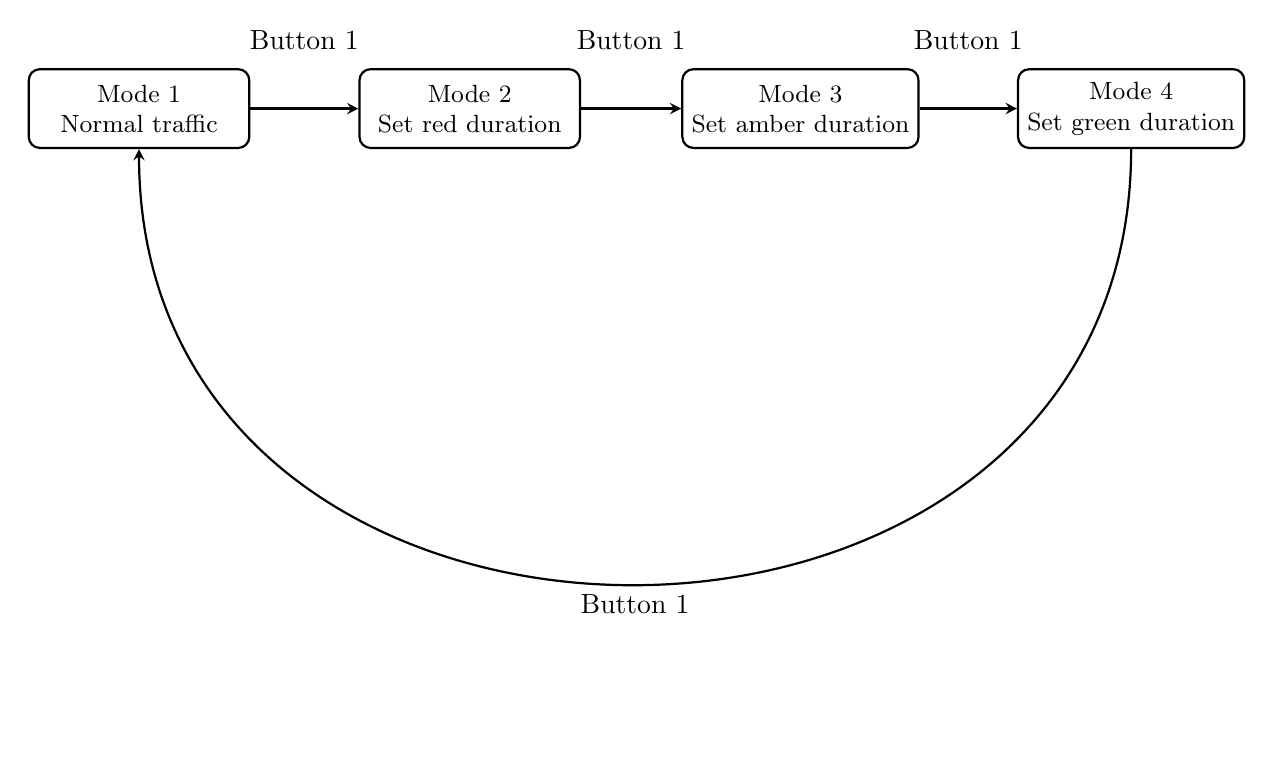
\begin{tikzpicture}[>=stealth, state/.style={draw, rounded corners, align=center, minimum width=2.8cm, minimum height=1.0cm, font=\small}, every path/.style={thick}]
        \node[state] (m1) at (0,0) {Mode 1\\Normal traffic};
        \node[state] (m2) at (4.2,0) {Mode 2\\Set red duration};
        \node[state] (m3) at (8.4,0) {Mode 3\\Set amber duration};
        \node[state] (m4) at (12.6,0) {Mode 4\\Set green duration};
        \draw[->] (m1.east) -- node[midway,above,yshift=20pt,draw=none,fill=white,inner sep=1pt] {Button 1} (m2.west);
        \draw[->] (m2.east) -- node[midway,above,yshift=20pt,draw=none,fill=white,inner sep=1pt] {Button 1} (m3.west);
        \draw[->] (m3.east) -- node[midway,above,yshift=20pt,draw=none,fill=white,inner sep=1pt] {Button 1} (m4.west);
        \draw[->] (m4.south) to[out=-90,in=-90,looseness=1.5] node[below,draw=none] {Button 1} (m1.south);
    \end{tikzpicture}%
    }
    \caption{Mode-selection FSM}
    \label{fig:exercise1_mode_fsm}
\end{figure}

Button 1 advances through Mode 1, Mode 2, Mode 3, and Mode 4, then returns to Mode 1. In a configuration mode, a short Button 2 press increases the selected timing value, a long press decreases it, and Button 3 confirms the value. The long-press behavior is an addition in the supplied source code; the lab specification explicitly requires increasing and confirming the value.

\subsection*{2.2 Normal traffic-phase FSM}
\begin{figure}[H]
    \centering
    \resizebox{\textwidth}{!}{%
    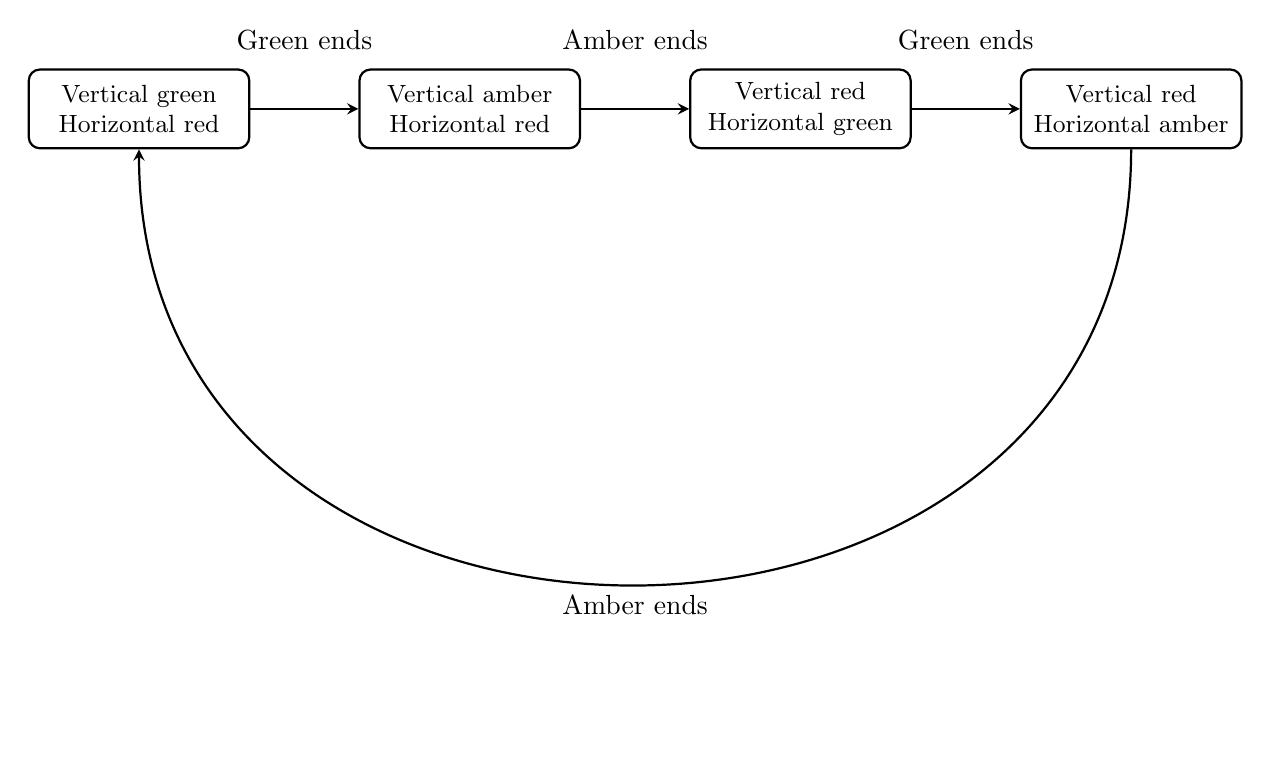
\begin{tikzpicture}[>=stealth, state/.style={draw, rounded corners, align=center, minimum width=2.8cm, minimum height=1.0cm, font=\small}, every path/.style={thick}]
        \node[state] (p1) at (0,0) {Vertical green\\Horizontal red};
        \node[state] (p2) at (4.2,0) {Vertical amber\\Horizontal red};
        \node[state] (p3) at (8.4,0) {Vertical red\\Horizontal green};
        \node[state] (p4) at (12.6,0) {Vertical red\\Horizontal amber};
        \draw[->] (p1.east) -- node[midway,above,yshift=20pt,draw=none,fill=white,inner sep=1pt] {Green ends} (p2.west);
        \draw[->] (p2.east) -- node[midway,above,yshift=20pt,draw=none,fill=white,inner sep=1pt] {Amber ends} (p3.west);
        \draw[->] (p3.east) -- node[midway,above,yshift=20pt,draw=none,fill=white,inner sep=1pt] {Green ends} (p4.west);
        \draw[->] (p4.south) to[out=-90,in=-90,looseness=1.5] node[below,draw=none] {Amber ends} (p1.south);
    \end{tikzpicture}%
    }
    \caption{Traffic-phase FSM used in Mode 1}
    \label{fig:exercise1_traffic_fsm}
\end{figure}

The phase sequence starts with the vertical road green and the horizontal road red. Each green phase is followed by its amber phase; after the amber duration expires, the other road receives the green signal. The sequence repeats continuously. The phase duration is read from the configured green or amber value.

\vspace{0.2cm}
\begin{resultbox}
The FSM separates user-interface behavior from traffic-phase behavior. This makes mode changes and timing configuration easier to reason about, while keeping the traffic sequence deterministic in normal mode.
\end{resultbox}
